\subsection{Statistique descriptive en 2D}


\subsubsection{Covariance}

\begin{center}
	\begin{tabular}{cc}
		\multicolumn{2}{c}{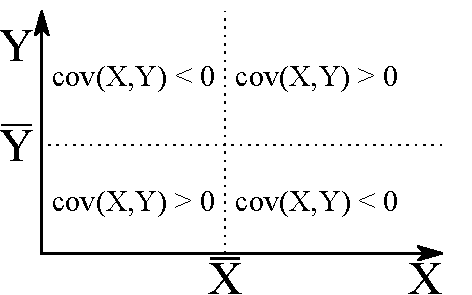
\includegraphics[width=0.3\textwidth]{images/covariance-all.pdf}}\\
		\multicolumn{2}{c}{Allure générale}\\
		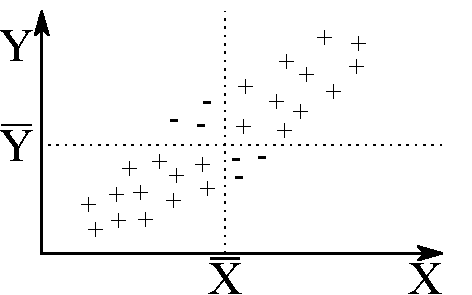
\includegraphics[width=0.3\textwidth]{images/covariance-positive.pdf}&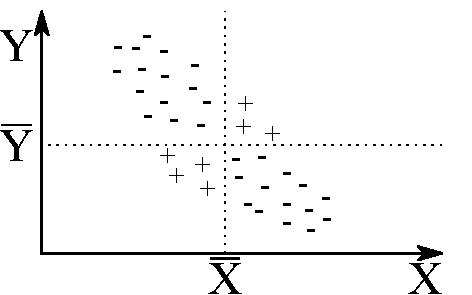
\includegraphics[width=0.3\textwidth]{images/covariance-negative.pdf}\\
		$n_{11}>0$&$n_{11}<0$
	\end{tabular}
\end{center}





\paragraph{La covariance $|m_{11}| \leq s_1s_2$}

La covariance est le moment d'ordre (1,1):

$$m_{11}=\frac{1}{n} \sum_{i=1}^{p} \sum_{j=1}^{q} n_{ij} (x_i-\bar{x})(y_j-\bar{y})$$

\begin{align}
\alpha  &= \label{carre} \frac{1}{n} \sum_{i=1}^{p} \sum_{j=1}^{q} n_{ij} ((x_i-\bar{x})(y_j-\bar{y}))^2 \\
        &= \frac{1}{n} \sum_{i=1}^{p} \sum_{j=1}^{q} n_{ij} (u^2(x_i-\bar{x})^2 + 2a(x_i-\bar{x})(y_j-\bar{y})+(y_j-\bar{y})^2)\\
        &= u^2s_1^2+2u\ m_{11}+s_2^2
\end{align}

L'équation~\eqref{carre} est au carré car toujours $\geq 0$.

\begin{align*}
\Delta &\leq 0\\
m_{11}^2-s_1^2s_2^2 &\leq 0\\
m_{11}^2 &\leq s_1^2s_2^2\\
|m_{11}| &\leq s_1s_2
\end{align*}




\paragraph{La covariance maximale $|m_{11}| = s_1s_2$}

La valeur absolue de la covariance est maximaleet vaut $|m_{11}| = s_1s_2$.

Si les points observés se trouvent sur une droite $ax+bx+c=0$, on a $ax_i+by_i+c=0$.

On multiplie par $\frac{n_{ij}}{n}$ et on somme sur $ij$.

\begin{align}
0  &= \sum_{i=1}^{p} \sum_{j=1}^{q} \frac{n_{ij}}{n}(ax_i+by_j+c) \\
   &= a \frac{1}{n} \sum_{i=1}^{p} \sum_{j=1}^{q}n_{ij}x_i + b \frac{1}{n} \sum_{i=1}^{p} \sum_{j=1}^{q}n_{ij}y_j + c \frac{1}{n} \sum_{i=1}^{p} \sum_{j=1}^{q}n_{ij}\\
   &= a\bar{x}+b\bar{y}+c\\
\intertext{On soustrait $ax_i+by_j+c=0$ par $a\bar{x}+b\bar{y}+c = 0$.}
   &= a(x_i-\bar{x})+b(y_j+\bar{y})\\
\intertext{On utilise $u_0=\frac{a}{b}$}
   &= u_0b(x_i-\bar{x})+\frac{a}{u_0}(y_j-\bar{y})\\
   &= u_0b(x_i-\bar{x})+\frac{u_0b}{u_0}(y_j-\bar{y})\\
   &= \label{max_covariance}u_0(x_i-\bar{x})+(y_j-\bar{y})
\end{align}

L'équation \eqref{max_covariance} a la même forme que $\alpha$, du coup...
\begin{align*}
0  &= \Delta\\
        &= m_{11}^2-s_1^2s_2^2\\
m_{11}^2 &= s_1^2s_2^2\\
|m_{11}| &= s_1s_2
\end{align*}




\subsubsection{Le coefficient de corrélation}
$$r=\frac{m_{11}}{s_1s_2}$$



\subsubsection{Les droites de régression}

\begin{center}
	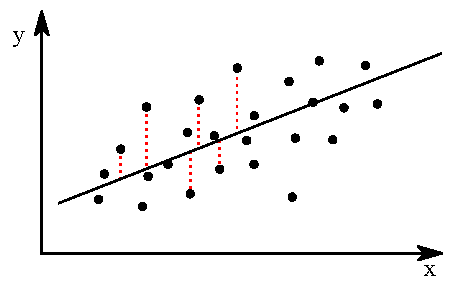
\includegraphics[width=0.3\textwidth]{images/droite_de_regression.pdf}
\end{center}
La droite de régression de y en x est la droite qui minimise la somme des carrés des écarts (parallèles à l'axe y) des points observés à cette droite.
$$g(a,b) = \sum_{i=1}^{p} \sum_{j=1}^{q} n_{ij} (y_j - a\ x_i - b)^2$$

\begin{align}
g(a,b)|_a &= \sum_{i=1}^{p} \sum_{j=1}^{q} 2n_{ij}(y_j - a\ x_i-b)(-x_i)\\
          &= \sum_{i=1}^{p} \sum_{j=1}^{q} 2n_{ij}(-y_j + a\ x_i^2 + b\ x_i)
\end{align}

\begin{align}
g(a,b)|_b &= \sum_{i=1}^{p} \sum_{j=1}^{q} 2n_{ij}(y_j - a\ x_i-b)(-1)\\
          &= \sum_{i=1}^{p} \sum_{j=1}^{q} 2n_{ij}(-y_j + a\ x_i + b)
\end{align}


